\documentclass[11pt]{article}
\usepackage[margin=0.85in]{geometry}
\usepackage{graphicx}
\usepackage{float}
\usepackage{fontspec}
\usepackage{parskip}
\usepackage{hyperref}
\setmainfont{Times New Roman}
\setsansfont{Arial}
\hypersetup{colorlinks=true,linkcolor=black,urlcolor=blue}
\setlength{\parindent}{0pt}
\setlength{\parskip}{6pt}
\graphicspath{{./}}
\begin{document}
\begin{center}
{\LARGE COMPSCI 182 Homework 02}\\[8pt]
{\large Chenyang Zhang}
\end{center}
\vspace{0.2in}
\section*{1}
\subsection*{(a)}
\begin{figure}[H]
\centering
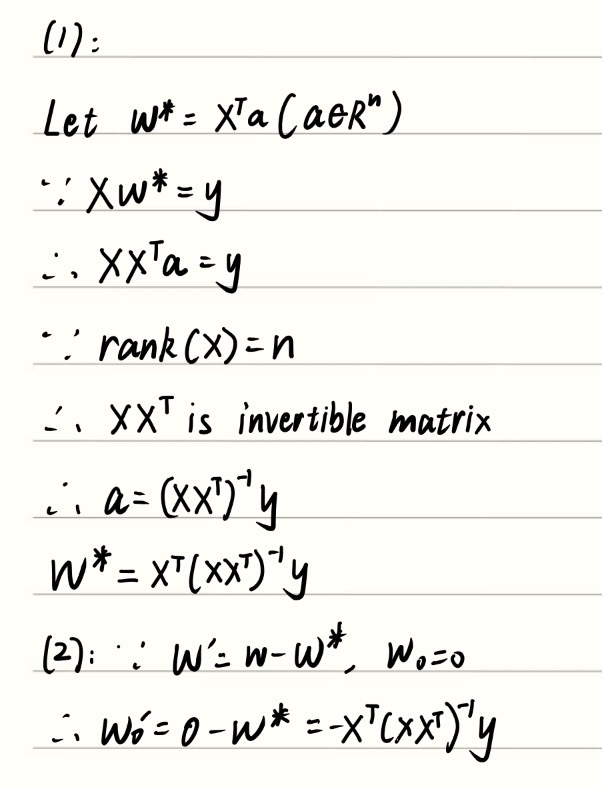
\includegraphics[width=0.96\textwidth,height=0.78\textheight,keepaspectratio]{assets/image_001.jpg}
\end{figure}

\subsection*{(b)}
\begin{figure}[H]
\centering
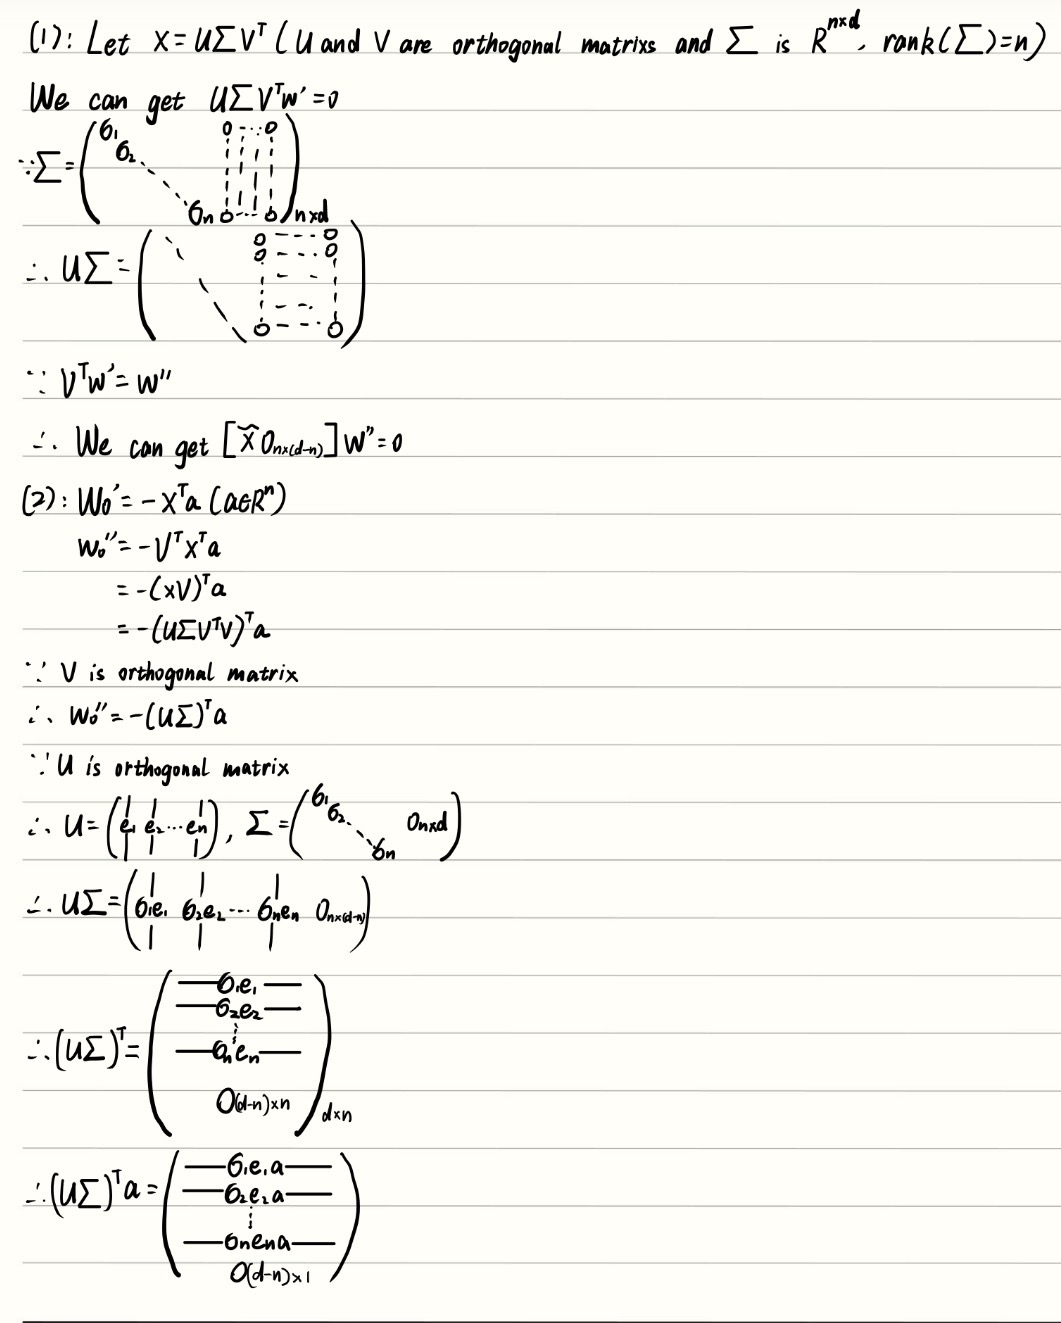
\includegraphics[width=0.96\textwidth,height=0.78\textheight,keepaspectratio]{assets/image_002.jpg}
\end{figure}

\subsection*{(c)}
\begin{figure}[H]
\centering
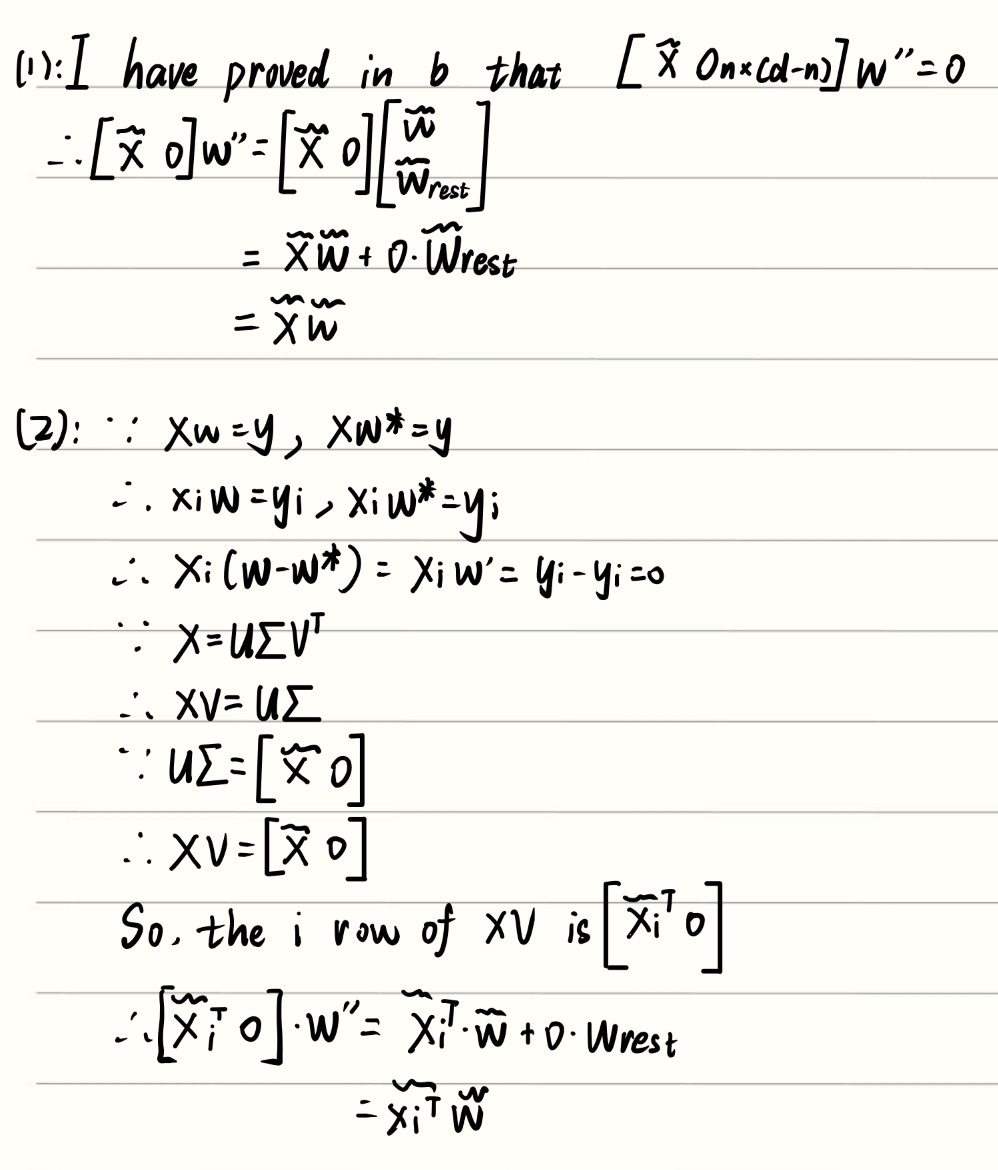
\includegraphics[width=0.96\textwidth,height=0.78\textheight,keepaspectratio]{assets/image_003.jpg}
\end{figure}

\subsection*{(d)}
\begin{figure}[H]
\centering
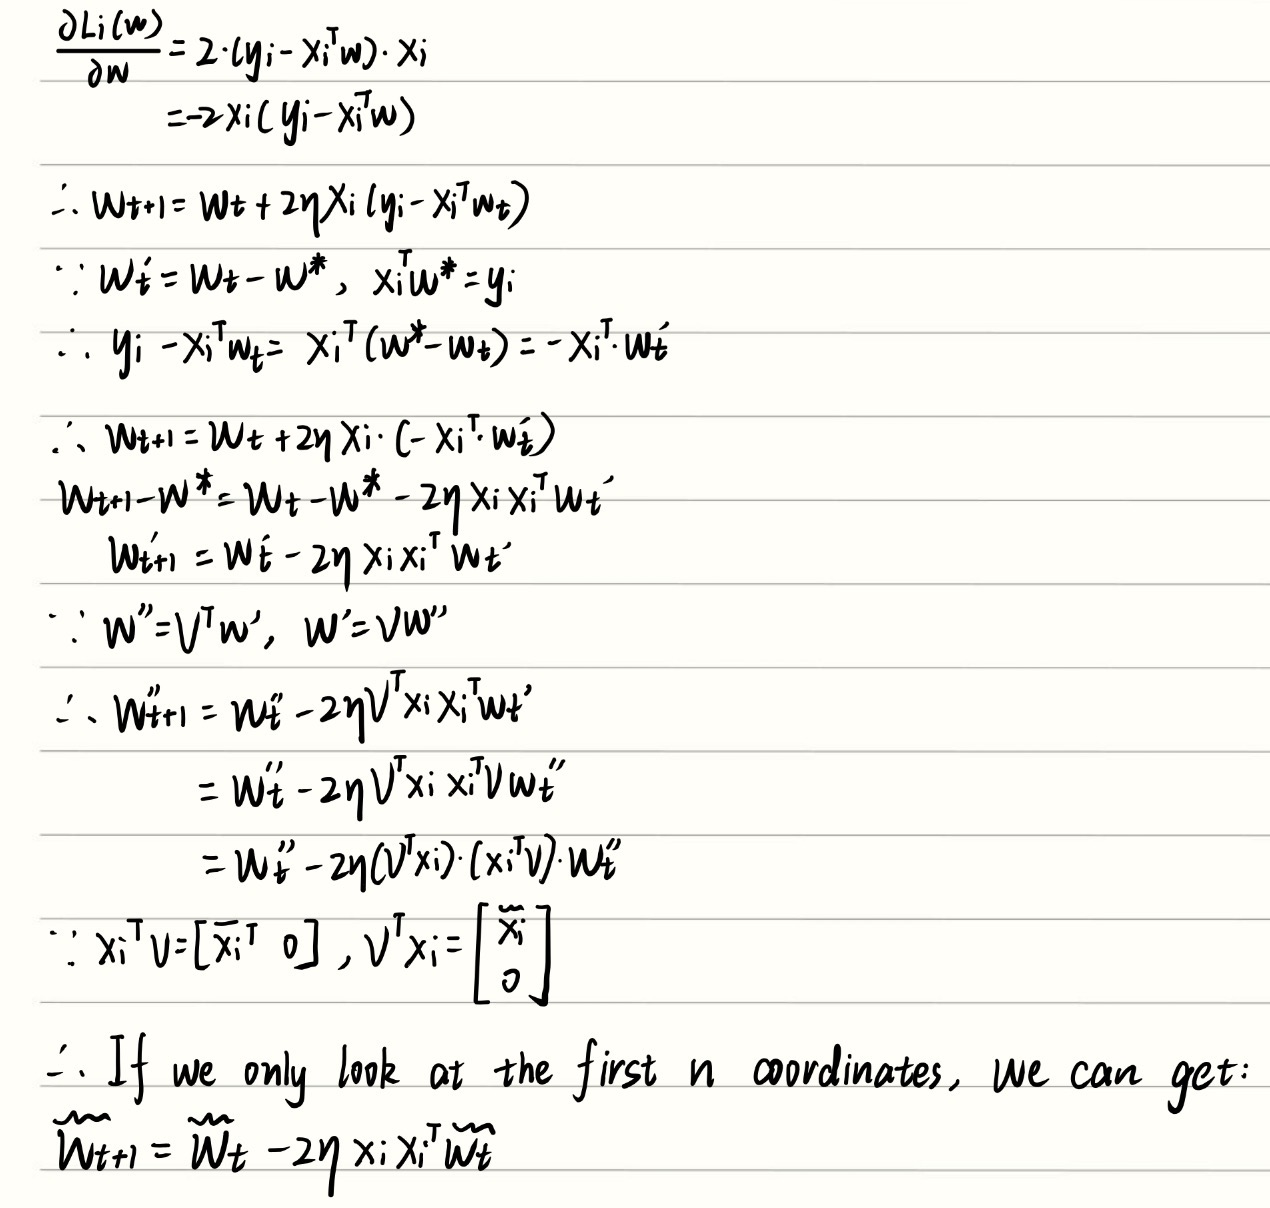
\includegraphics[width=0.96\textwidth,height=0.78\textheight,keepaspectratio]{assets/image_004.jpg}
\end{figure}

\subsection*{(e)}
\begin{figure}[H]
\centering
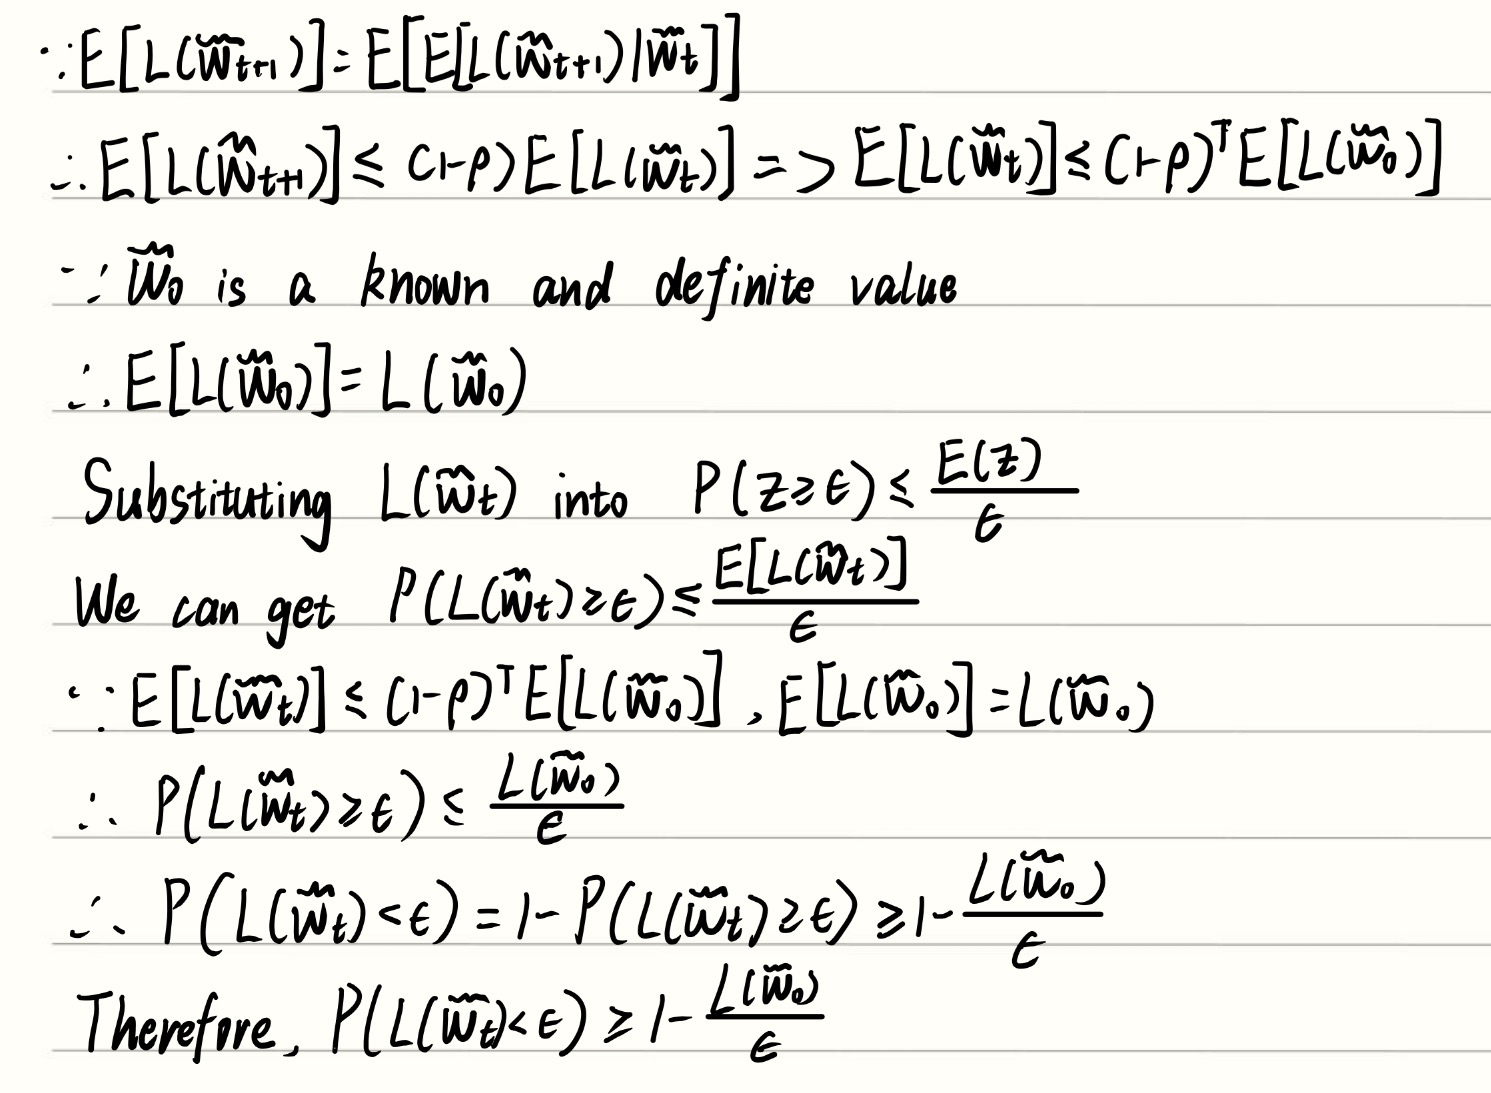
\includegraphics[width=0.96\textwidth,height=0.78\textheight,keepaspectratio]{assets/image_005.jpg}
\end{figure}

\subsection*{(f)}
\begin{figure}[H]
\centering
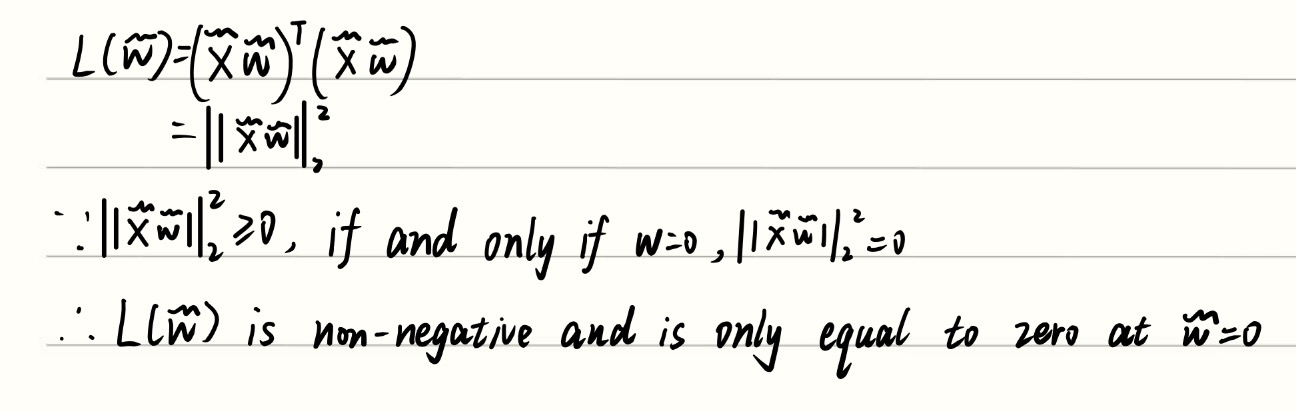
\includegraphics[width=0.96\textwidth,height=0.78\textheight,keepaspectratio]{assets/image_006.jpg}
\end{figure}

\subsection*{(g)}
\begin{figure}[H]
\centering
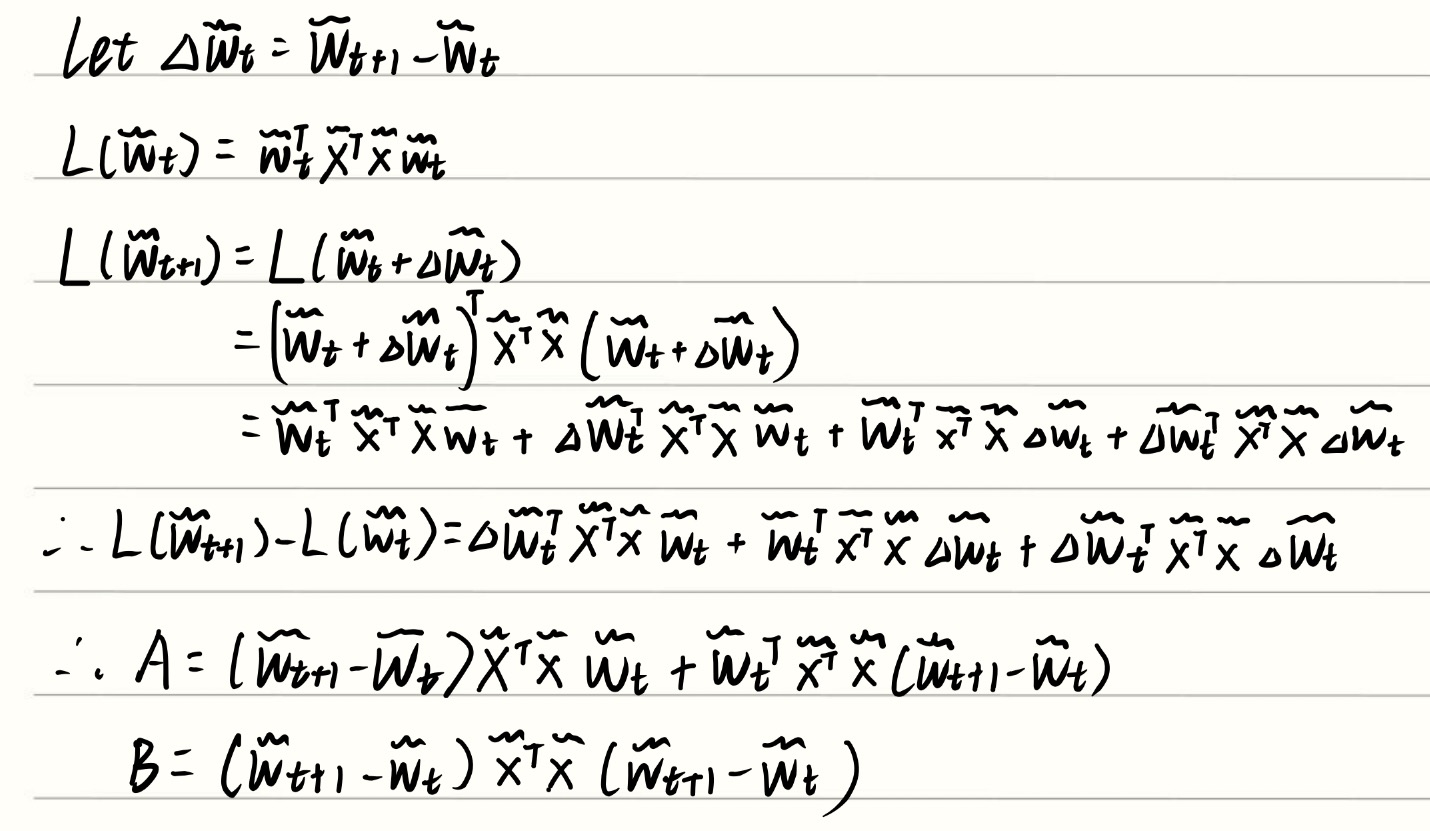
\includegraphics[width=0.96\textwidth,height=0.78\textheight,keepaspectratio]{assets/image_007.jpg}
\end{figure}

\subsection*{(h)}
\begin{figure}[H]
\centering
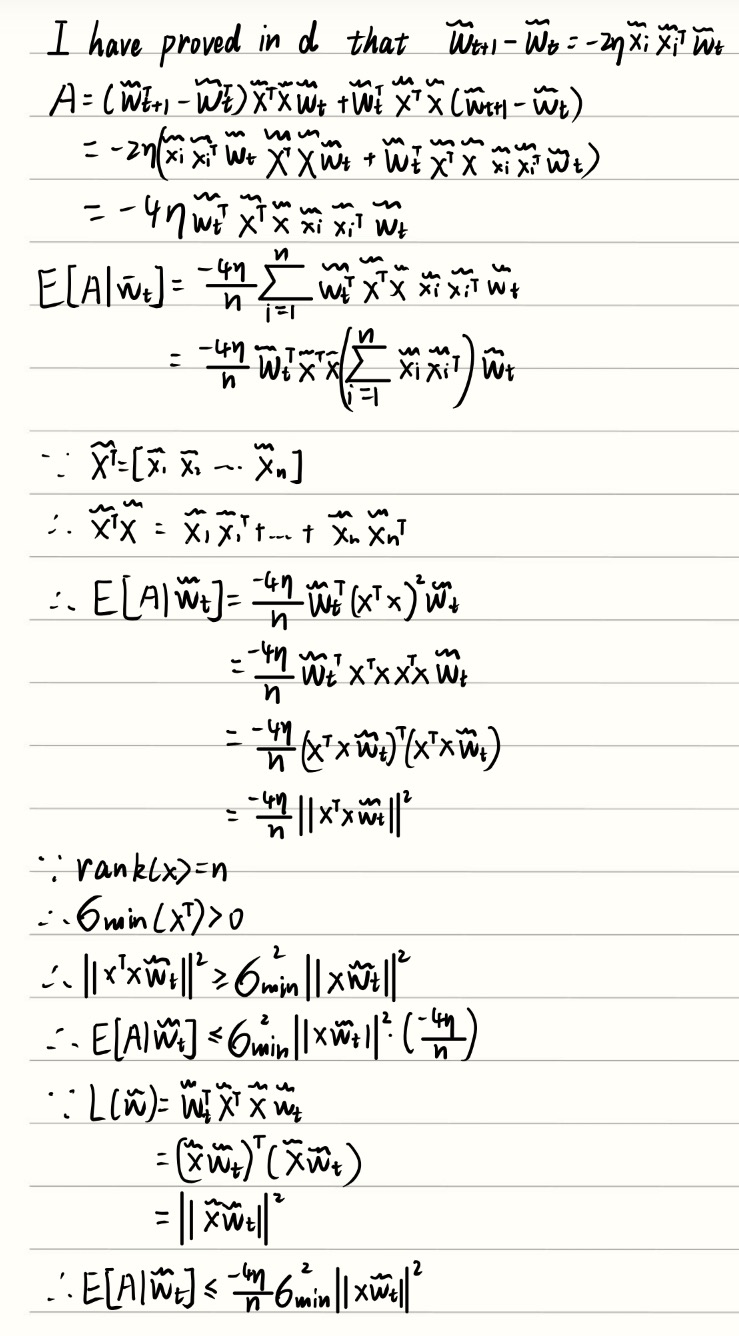
\includegraphics[width=0.96\textwidth,height=0.78\textheight,keepaspectratio]{assets/image_008.jpg}
\end{figure}

\subsection*{(i)}
\begin{figure}[H]
\centering
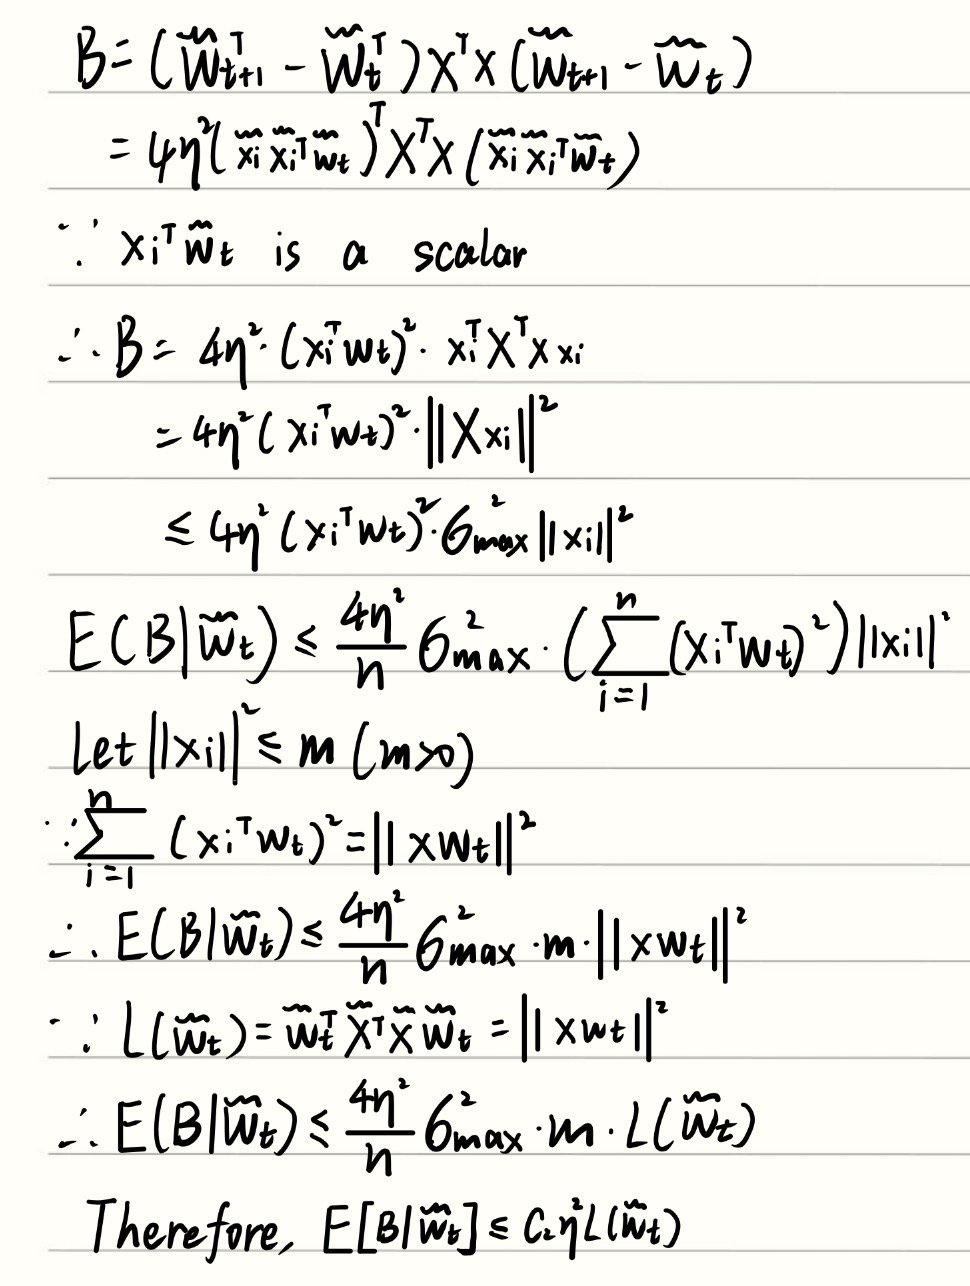
\includegraphics[width=0.96\textwidth,height=0.78\textheight,keepaspectratio]{assets/image_009.jpg}
\end{figure}

\subsection*{(j)}
\begin{figure}[H]
\centering
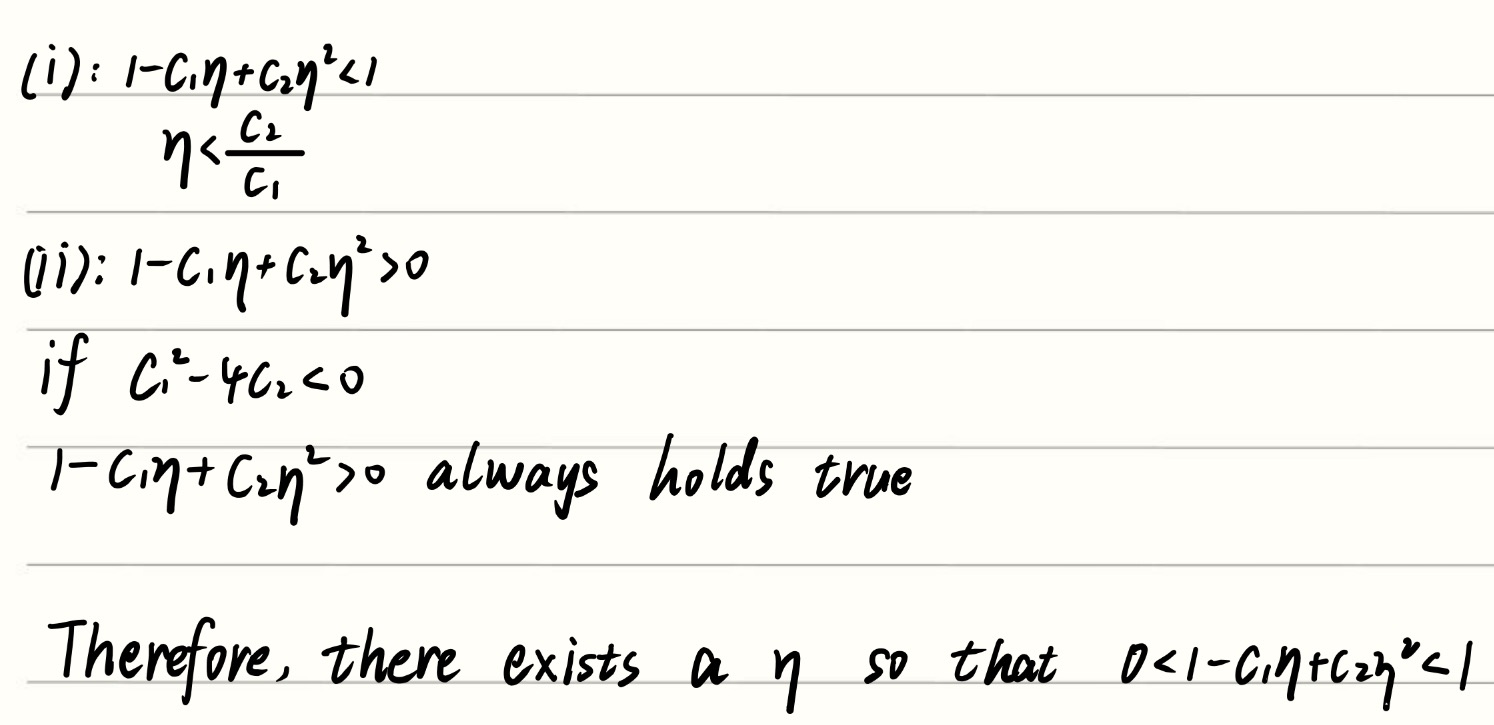
\includegraphics[width=0.96\textwidth,height=0.78\textheight,keepaspectratio]{assets/image_010.jpg}
\end{figure}

\subsection*{(k)}
The original ridge SGD decreases rapidly at first, but then fluctuates around a nonzero error level. In contrast, the feature-augmented SGD keeps decreasing and approaches zero. Thus, the feature-augmented method continues converging toward the ridge solution, while the original ridge SGD reaches a nonzero error floor.

\vspace{0.1in}\hrule\vspace{0.1in}
\section*{2}
\subsection*{(a)}
\begin{figure}[H]
\centering
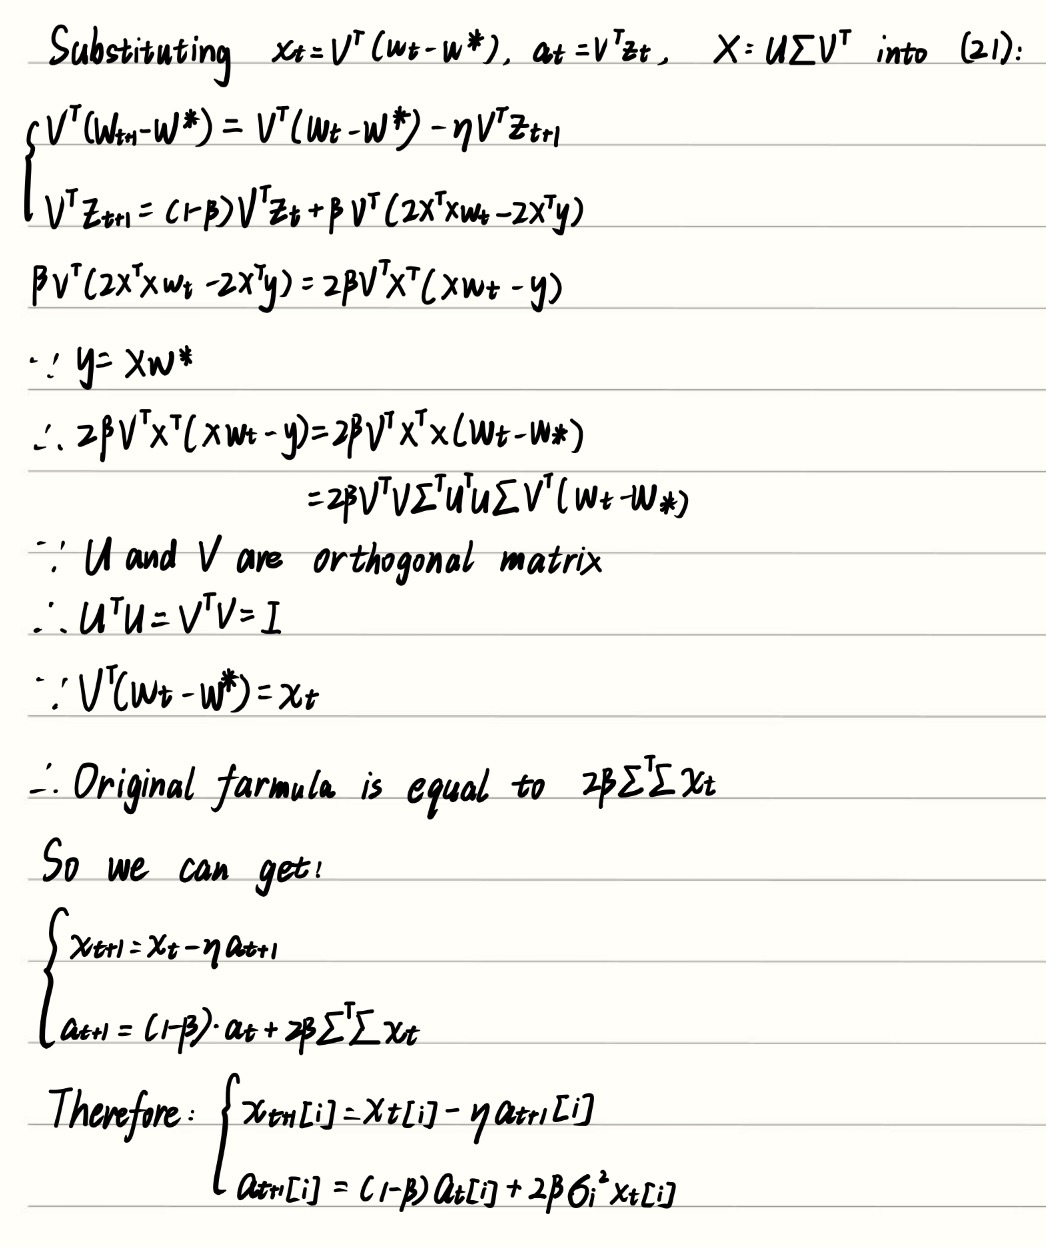
\includegraphics[width=0.96\textwidth,height=0.78\textheight,keepaspectratio]{assets/image_011.jpg}
\end{figure}

\subsection*{(b)}
\begin{figure}[H]
\centering
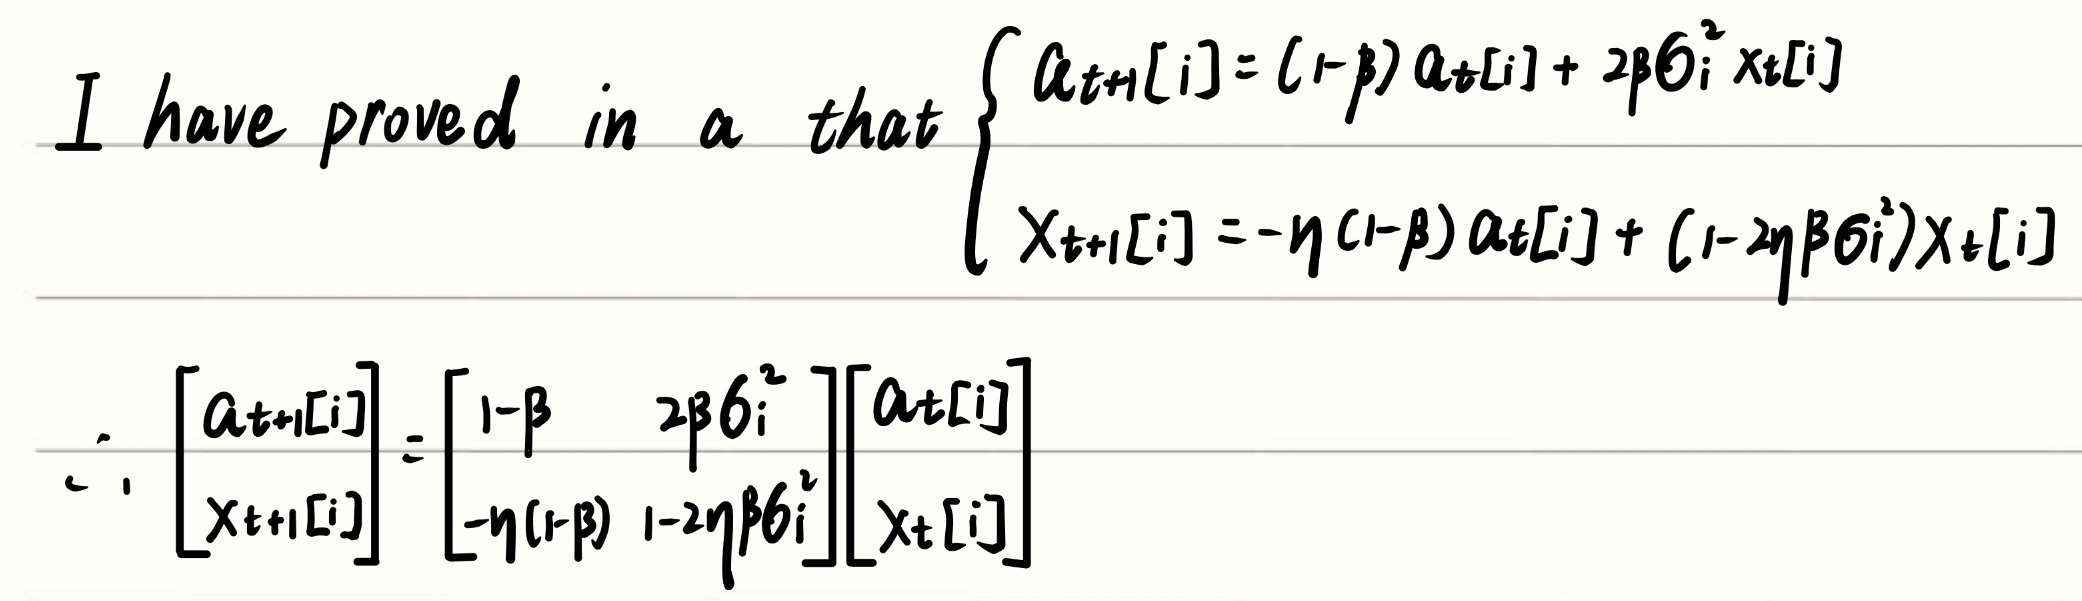
\includegraphics[width=0.96\textwidth,height=0.78\textheight,keepaspectratio]{assets/image_012.jpg}
\end{figure}

\subsection*{(c)}
\begin{figure}[H]
\centering
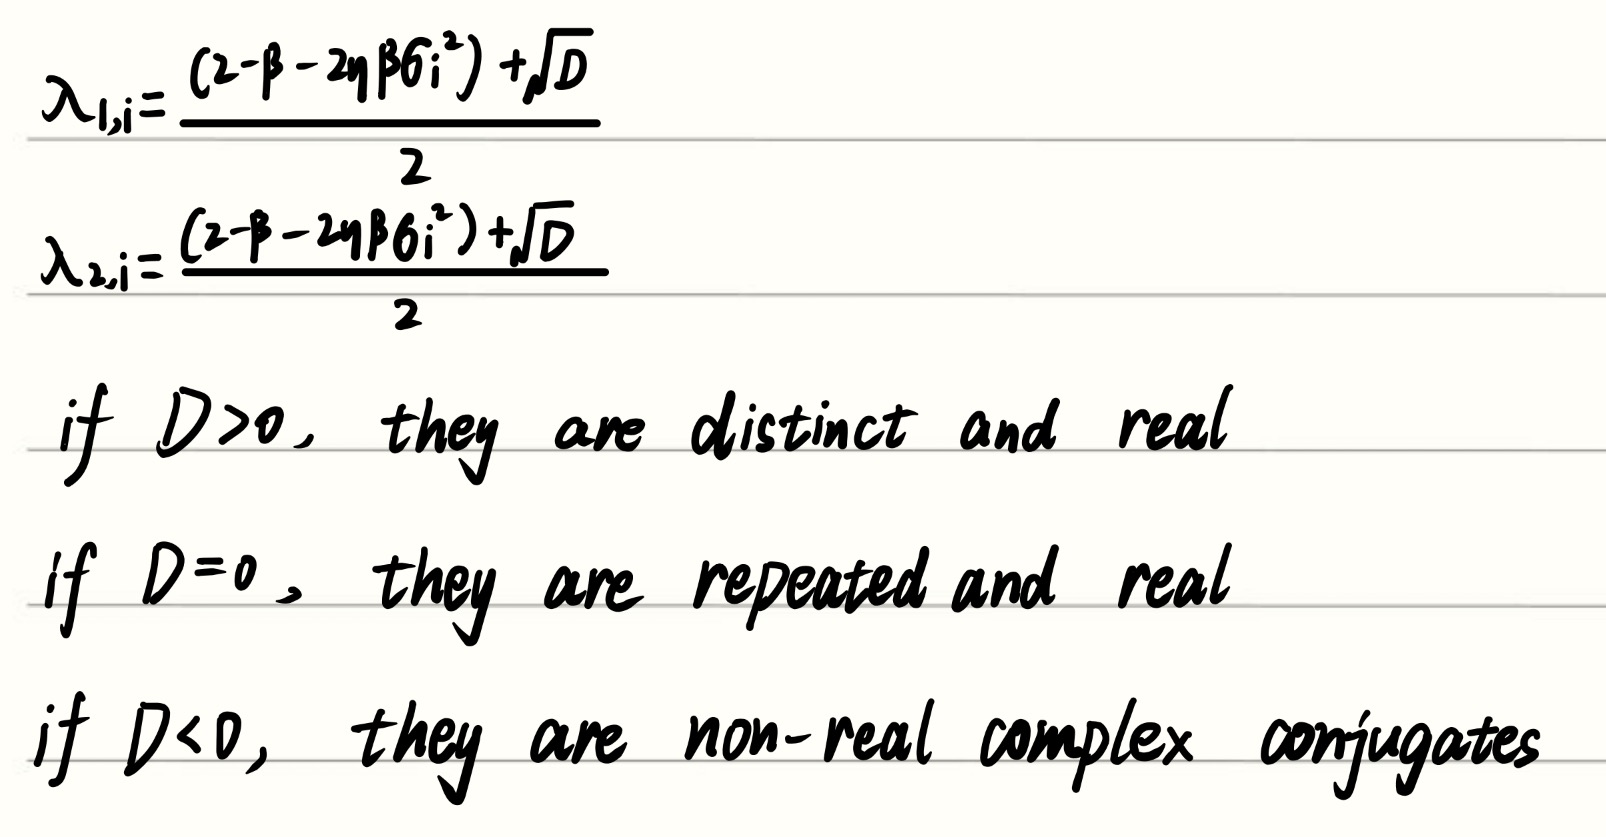
\includegraphics[width=0.96\textwidth,height=0.78\textheight,keepaspectratio]{assets/image_013.jpg}
\end{figure}

\subsection*{(d)}
\begin{figure}[H]
\centering
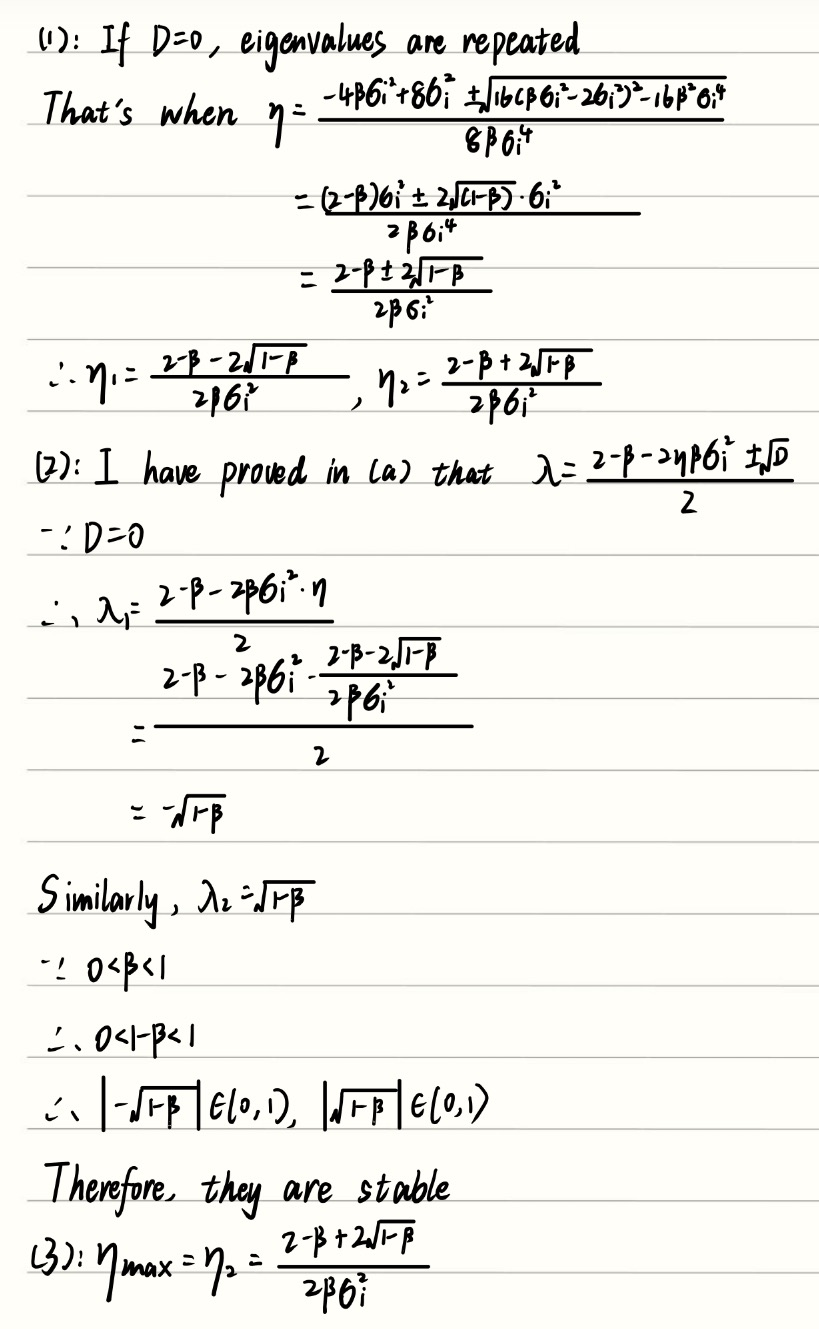
\includegraphics[width=0.96\textwidth,height=0.78\textheight,keepaspectratio]{assets/image_014.jpg}
\end{figure}

\subsection*{(e)}
\begin{figure}[H]
\centering
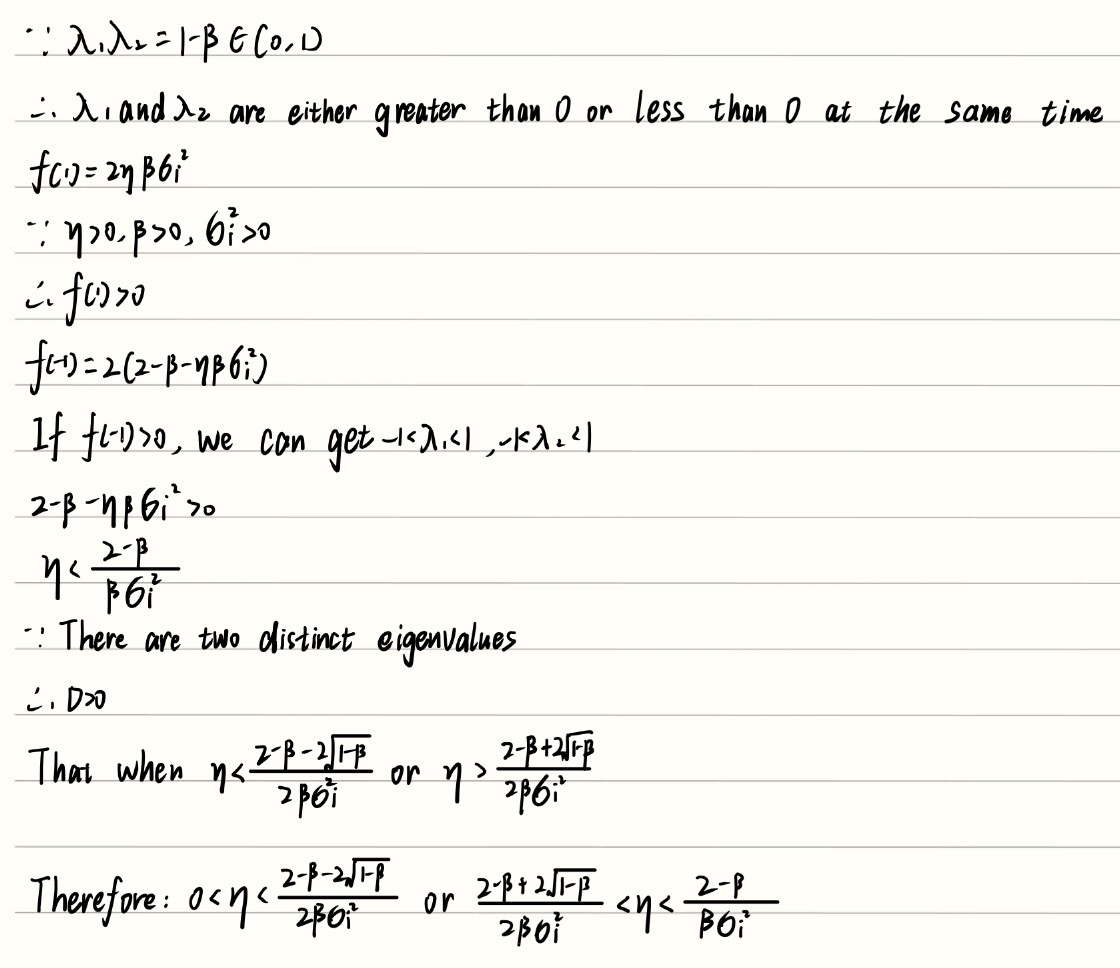
\includegraphics[width=0.96\textwidth,height=0.78\textheight,keepaspectratio]{assets/image_015.jpg}
\end{figure}

\subsection*{(g)}
\begin{figure}[H]
\centering
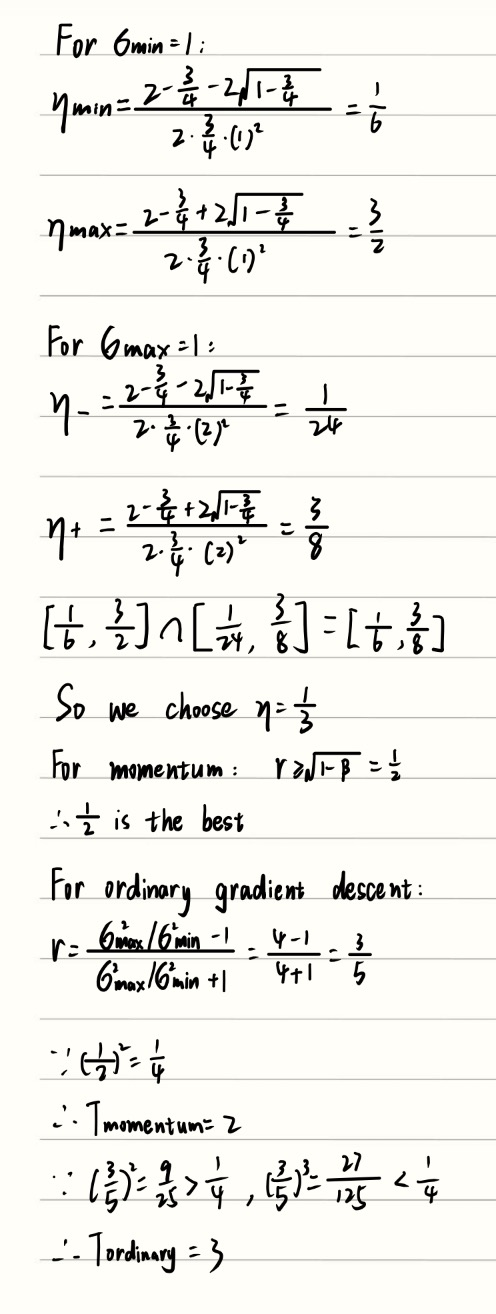
\includegraphics[width=0.96\textwidth,height=0.78\textheight,keepaspectratio]{assets/image_016.jpg}
\end{figure}

\subsection*{(h)}
Thus, directions with larger singular values are updated more aggressively, while directions with smaller singular values change more slowly.

\subsection*{(i)}
Gradient descent with momentum converges faster overall because momentum preserves part of the previous update direction, allowing the parameters to keep moving in a consistent direction instead of relying only on the current gradient.

\vspace{0.1in}\hrule\vspace{0.1in}
\section*{3}
\subsection*{(a)}
\begin{figure}[H]
\centering
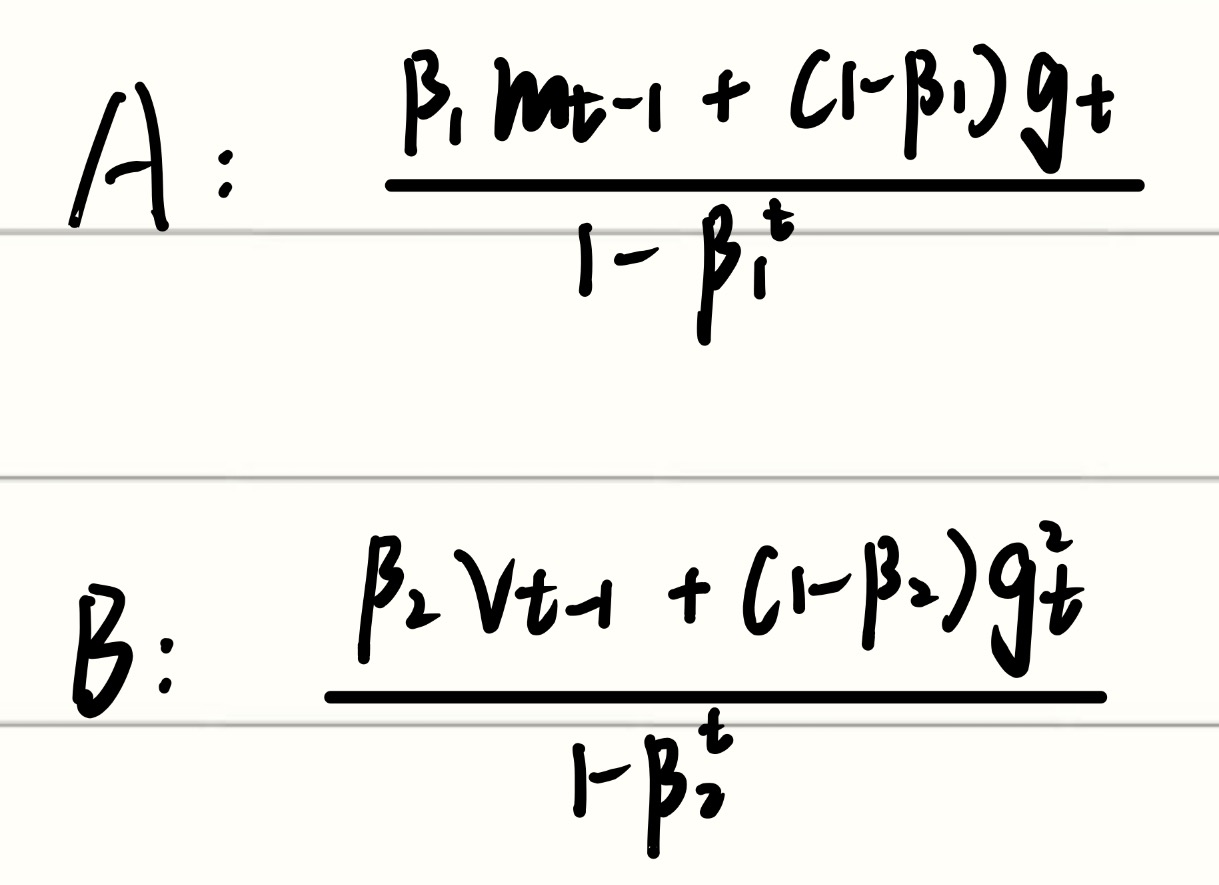
\includegraphics[width=0.96\textwidth,height=0.78\textheight,keepaspectratio]{assets/image_017.jpg}
\end{figure}

\subsection*{(b)}
\begin{figure}[H]
\centering
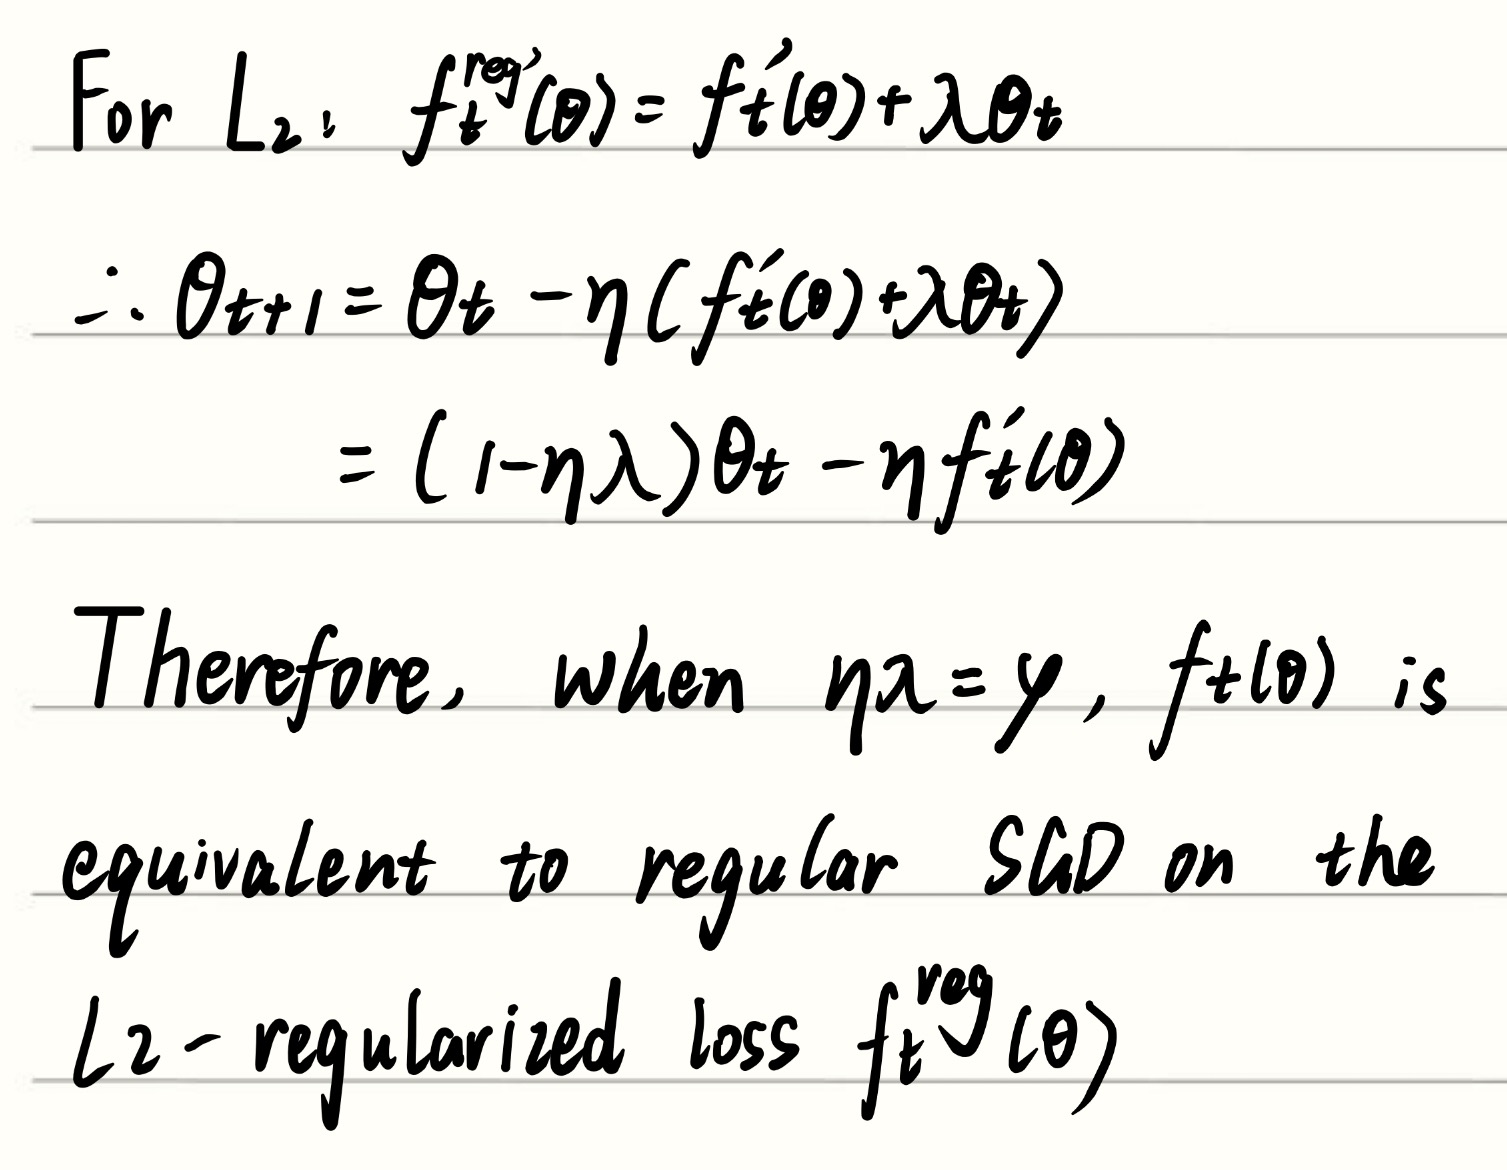
\includegraphics[width=0.96\textwidth,height=0.78\textheight,keepaspectratio]{assets/image_018.jpg}
\end{figure}

\vspace{0.1in}\hrule\vspace{0.1in}
\section*{4}
\subsection*{(a)}
\begin{figure}[H]
\centering
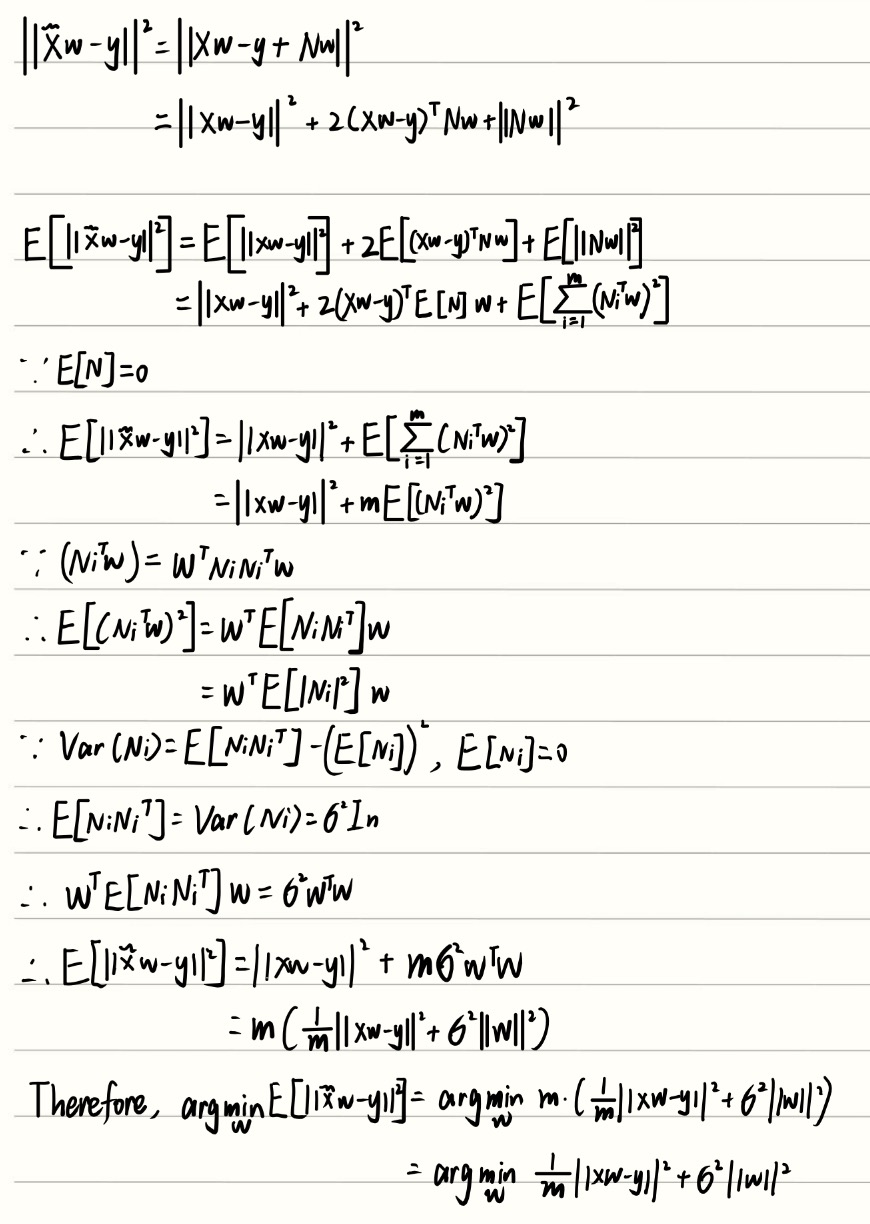
\includegraphics[width=0.96\textwidth,height=0.78\textheight,keepaspectratio]{assets/image_019.jpg}
\end{figure}

\subsection*{(b)}
\begin{figure}[H]
\centering
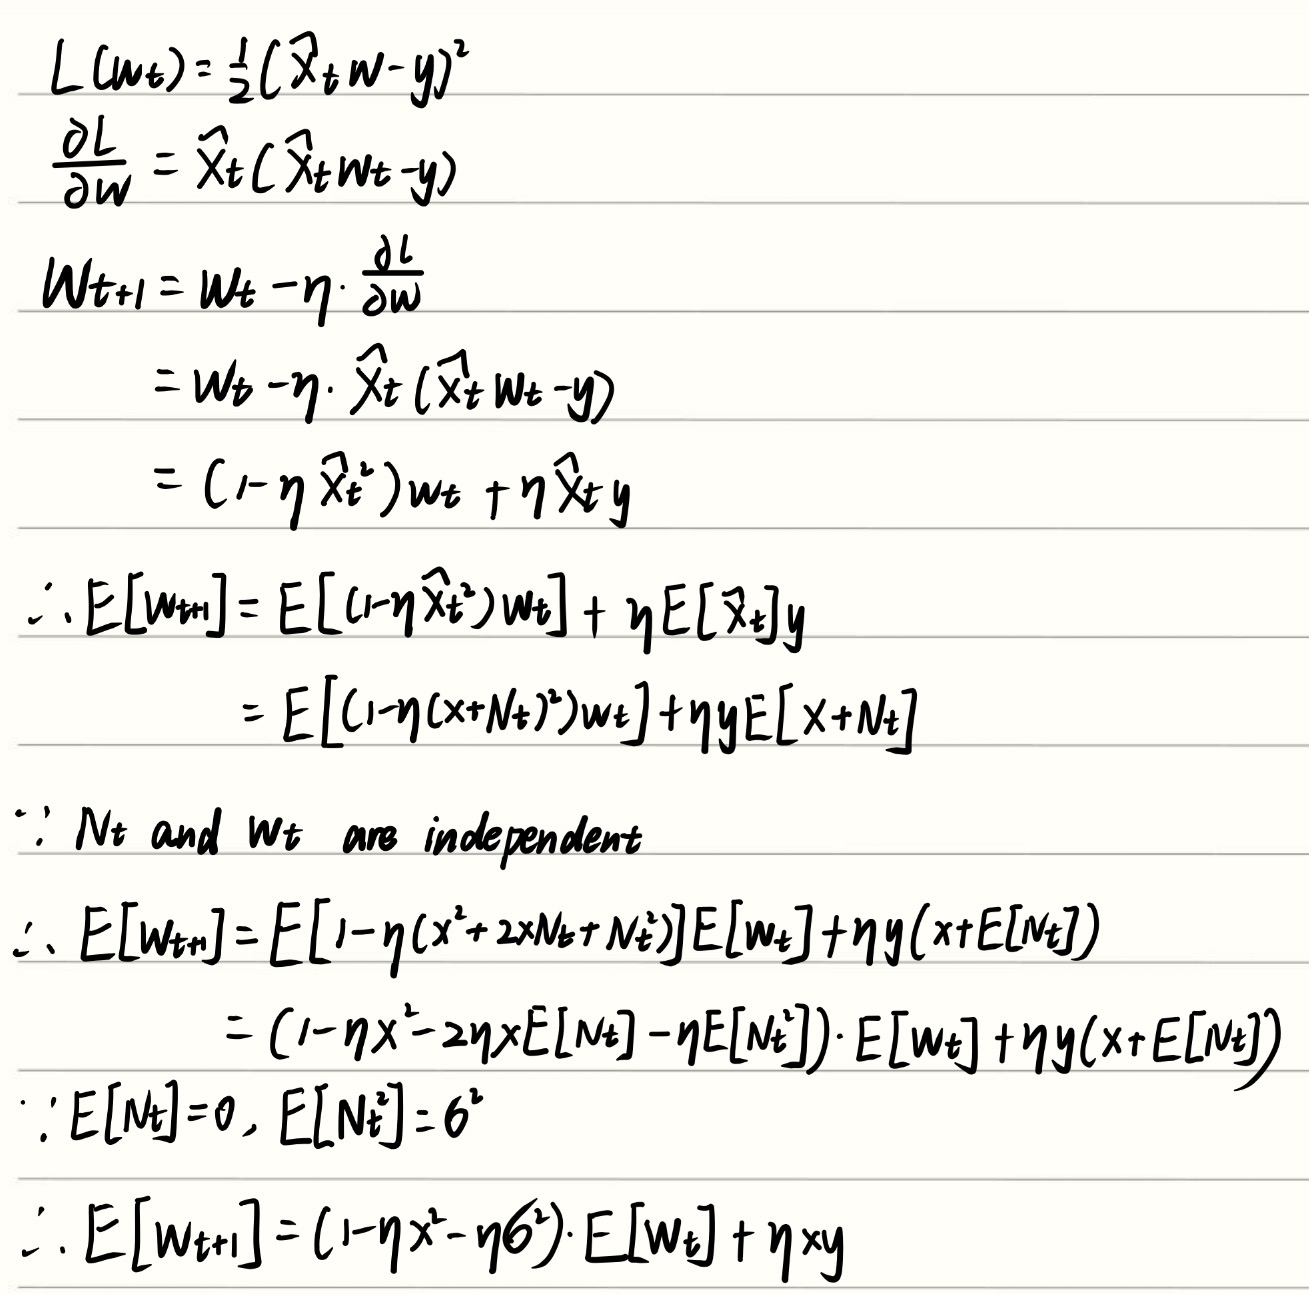
\includegraphics[width=0.96\textwidth,height=0.78\textheight,keepaspectratio]{assets/image_020.jpg}
\end{figure}

\subsection*{(c)}
\begin{figure}[H]
\centering
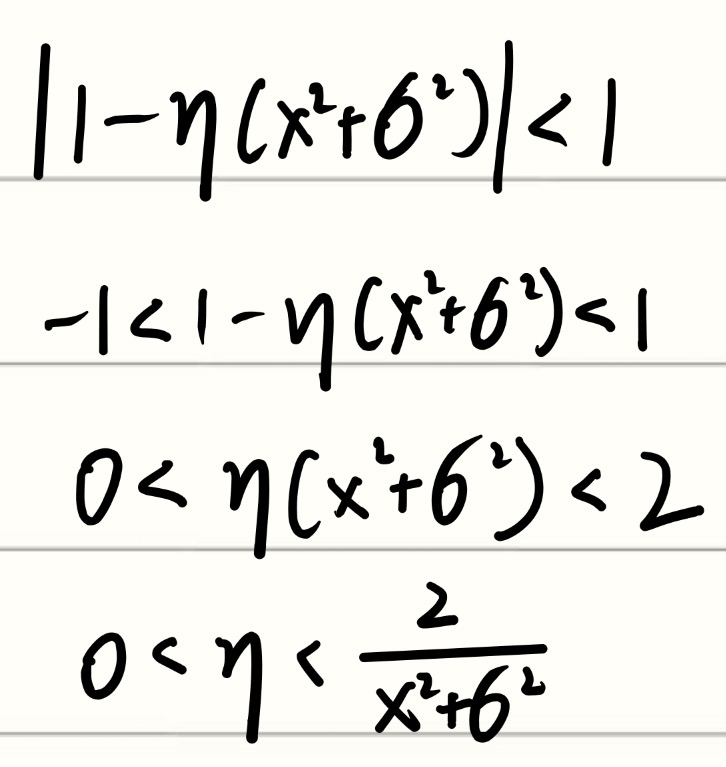
\includegraphics[width=0.96\textwidth,height=0.78\textheight,keepaspectratio]{assets/image_021.jpg}
\end{figure}

\subsection*{(d)}
\begin{figure}[H]
\centering
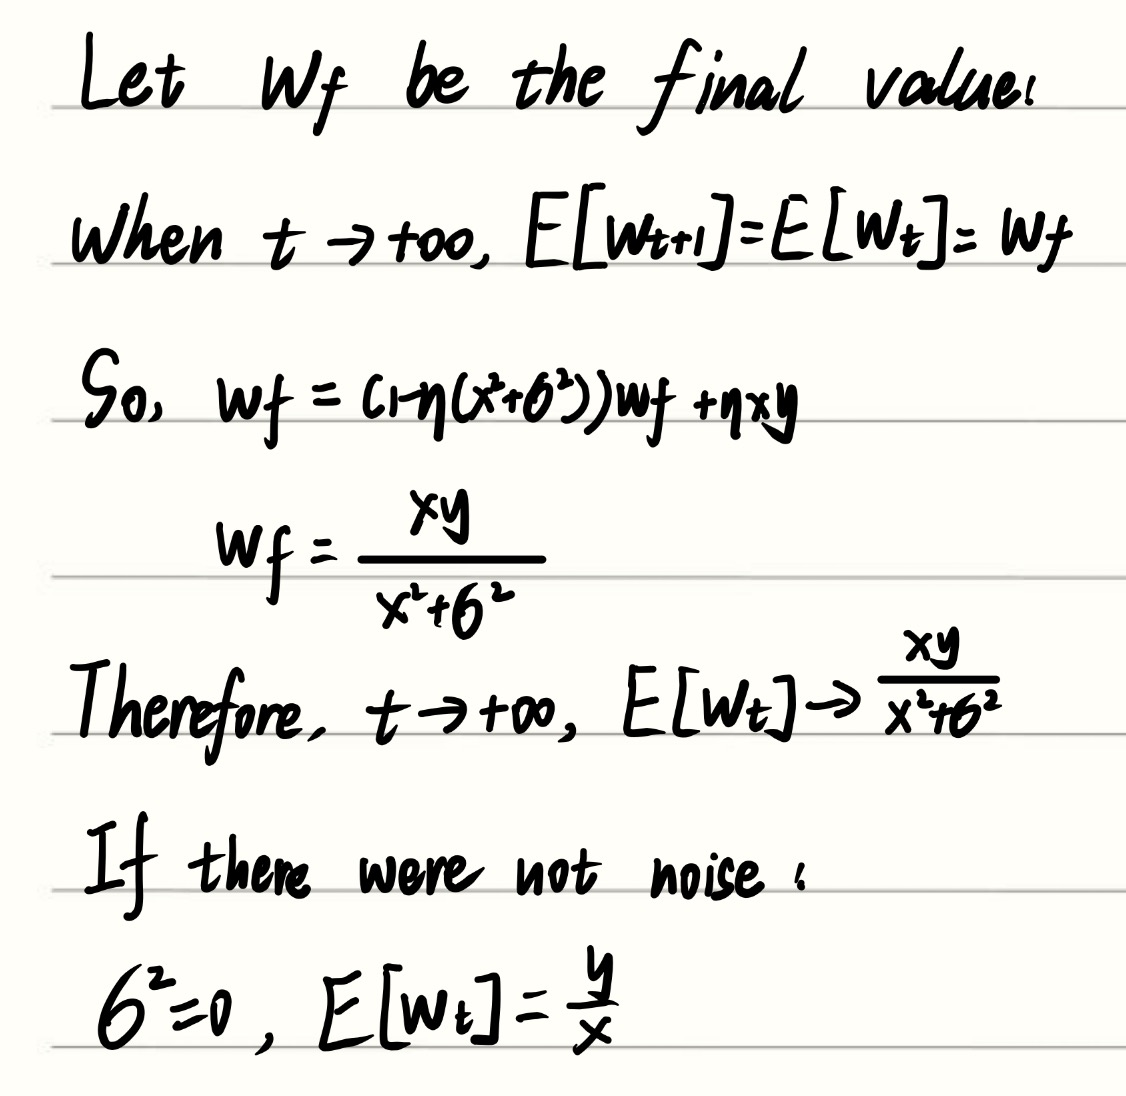
\includegraphics[width=0.96\textwidth,height=0.78\textheight,keepaspectratio]{assets/image_022.jpg}
\end{figure}

\vspace{0.1in}\hrule\vspace{0.1in}
\section*{5.}
See my answer in 2(h) and 2(i)

\end{document}